%%%%%%%%%%%%%%%%%%%%%%%%%%%%%%%%%%%%%%%%%%%%%%%%%%%%%%%%%%%%%%%%%%%%%%%%%%%%%%%
% Chapter 'Absorption - R-12 - paraffinic '
%%%%%%%%%%%%%%%%%%%%%%%%%%%%%%%%%%%%%%%%%%%%%%%%%%%%%%%%%%%%%%%%%%%%%%%%%%%%%%%
\subsection{Paraffinic }
%
%%%%%%%%%%%%%%%%%%%%%%%%%%%%%%%%%%%%%%%%%%%%%%%%%%%%%%%%%%%%%%%%%%%%%%%%%%%%%%%
%%%%%%%%%%%%%%%%%%%%%%%%%%%%%%%%%%%%%%%%%%%%%%%%%%%%%%%%%%%%%%%%%%%%%%%%%%%%%%%
\subsubsection{Heil - ID 1}
%
\begin{tabular}[l]{|lp{11.5cm}|}
\hline
\addlinespace

\textbf{Sorbent:} & paraffinic \\
\textbf{Subtype:} &  \\
\textbf{Refrigerant:} & R-12 \\
\textbf{Equation:} & Heil \\
\textbf{ID:} & 1 \\
\textbf{Reference:} & Grebner, J. J. (1992): The Effects of Oil on the Thermodynamic Properties of Dichlorodifluoromethane (R-12) and Tetrafluoroethane (R-134a). Hg. v. Air Conditioning and Refrigeration Center. College of Engineering. University of Illinois at Urbana-Champaign. Air Conditioning and Refrigeration Center TR-13. Online verfügbar unter http://hdl.handle.net/2142/9702. \\
\textbf{Comment:} & See original literature: Use low-level interface to input molar volumes of both components, which are calculated by propper equations of state (i.e., v\_POE =  1/((55.37-0.020428*((T-273.15)*1.8+32))*16.0185)*0.5 in m3/mol), for calculations. \\

\addlinespace
\hline
\end{tabular}
\newline

\textbf{Equation and parameters:}
\newline
%
Pressure $p$ in $\si{\pascal}$ is calculated depending on molar fraction of refrigerant in the liquid phase $x_1$ in $\si{\mole\per\mole}$, temperature $T$ in $\si{\kelvin}$, molar volumes of both components ($v_1$ and $v_2$) in $\si{\cubic\meter\per\mole}$, and vapor pressure $p_\mathrm{sat,1}$ in $\si{\pascal}$. If molar volumes less than zero are used as function arguements, constant molar volumes given by parameter record are used. Equilibrium equation is given by:
%
\begin{equation*}
\begin{split}
p &=& \gamma_1 x_1 p_\mathrm{sat,1} & \quad\text{, and} \\
\gamma_1 &=& \exp \left( - \ln \left( x_1 + \Lambda_{21} x_2 \right) + x_2 \left( \frac{\Lambda_{21}}{x_1 + \Lambda_{21} x_2} - \frac{\Lambda_{12}}{x_1 \Lambda_{12} + x_2} \right) + \Phi \right) & \quad\text{, and} \\
\Phi &=& x_2^2 \left( \tau_{12} \left( \frac{\Lambda_{21}}{x_1 + \Lambda_{21} x_2} \right) ^2 + \tau_{12} \frac{\Lambda_{12}}{\left( x_1 \Lambda_{12} + x_2 \right) ^2}  \right) & \quad\text{, and} \\
\Delta\Lambda_{12} &=& \nicefrac{v_2}{v_1} \exp \left( - \tau_{12} \right) & \quad\text{, and} \\
\Delta\Lambda_{21} &=& \nicefrac{v_1}{v_2} \exp \left( - \tau_{21} \right) & \quad\text{, and} \\
\tau_{12} &=& \nicefrac{\lambda_{12}}{R T} & \quad\text{, and} \\
\tau_{21} &=& \nicefrac{\lambda_{21}}{R T} & \quad\text{, and} \\
x_2 &=& 1 - x_1  & \quad\text{.} \\
\end{split}
\end{equation*}
%
The parameters of the equation are:
%
\begin{longtable}[l]{lll|lll}
\toprule
\addlinespace
\textbf{Par.} & \textbf{Unit} & \textbf{Value} &	\textbf{Par.} & \textbf{Unit} & \textbf{Value} \\
\addlinespace
\midrule
\endhead

\bottomrule
\endfoot
\bottomrule
\endlastfoot
\addlinespace

$\Delta\lambda_{12}$ & $\si{\joule\per\mole}$ & 1.307000000e+03 & $\Delta\lambda_{21}$ & $\si{\joule\per\mole}$ & 1.615000000e+03 \\
$v_1$ & $\si{\cubic\meter\per\mole}$ & 1.000000000e+00 & $v_2$ & $\si{\cubic\meter\per\mole}$ & 1.000000000e+00 \\

\addlinespace\end{longtable}

\textbf{Validity:}
\newline
Equation is approximately valid for $255.15 \si{\kelvin} \leq T \leq 394.15 \si{\kelvin}$.
\newline

\textbf{Visualization:}
%
\begin{figure}[!htp]
{\noindent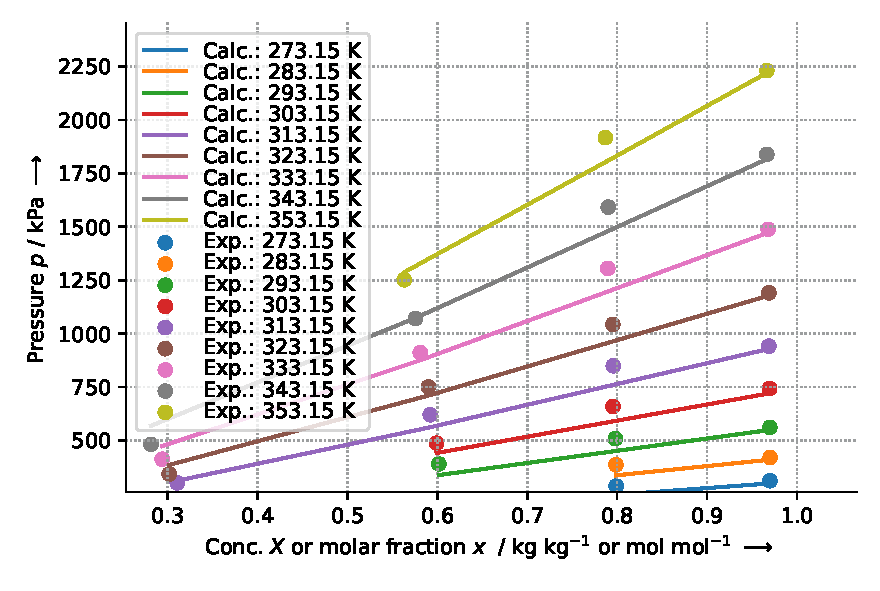
\includegraphics[height=10cm, keepaspectratio]{figs/abs/abs_R-12_paraffinic__Heil_1.pdf}}
\end{figure}
%

To generate the figure, the following refrigerant functions were selected:
\begin{itemize}
\item Vapor pressure: VaporPressure\_EoS1 - ID 1
\item Saturated liquid density: SaturatedLiquidDensity\_EoS1 - ID 1
\item Special refrigerant functions as described by comment and CoolProp
\end{itemize}

The uncertainity of the experimental data is:
\begin{itemize}
\item Data source $\,\to\,$ Data was taken from figure
\item Pressure, absolute, in $\si{\pascal}$ $\,\to\,$ 3.45E+02
\item Temperature, absolute, in $\si{\kelvin}$ $\,\to\,$ 0.12
\end{itemize}

The mean absolute percentage error (MAPE) between the experimental and calculated data results in 6.83\%.
\FloatBarrier
\newpage
%%%%%%%%%%%%%%%%%%%%%%%%%%%%%%%%%%%%%%%%%%%%%%%%%%%%%%%%%%%%%%%%%%%%%%%%%%%%%%%
%%%%%%%%%%%%%%%%%%%%%%%%%%%%%%%%%%%%%%%%%%%%%%%%%%%%%%%%%%%%%%%%%%%%%%%%%%%%%%%
\subsubsection{NrtlFixedDg - ID 1}
%
\begin{tabular}[l]{|lp{11.5cm}|}
\hline
\addlinespace

\textbf{Sorbent:} & paraffinic \\
\textbf{Subtype:} &  \\
\textbf{Refrigerant:} & R-12 \\
\textbf{Equation:} & NrtlFixedDg \\
\textbf{ID:} & 1 \\
\textbf{Reference:} & Grebner, J. J. (1992): The Effects of Oil on the Thermodynamic Properties of Dichlorodifluoromethane (R-12) and Tetrafluoroethane (R-134a). Hg. v. Air Conditioning and Refrigeration Center. College of Engineering. University of Illinois at Urbana-Champaign. Air Conditioning and Refrigeration Center TR-13. Online verfügbar unter http://hdl.handle.net/2142/9702. \\
\textbf{Comment:} & None \\

\addlinespace
\hline
\end{tabular}
\newline

\textbf{Equation and parameters:}
\newline
%
Pressure $p$ in $\si{\pascal}$ is calculated depending on molar fraction of refrigerant in the liquid phase $x_1$ in $\si{\mole\per\mole}$, temperature $T$ in $\si{\kelvin}$, and vapor pressure $p_\mathrm{sat,1}$ in $\si{\pascal}$ by:
%
\begin{equation*}
\begin{split}
p &=& \gamma_1 x_1 p_\mathrm{sat,1} & \quad\text{, and} \\
\gamma_1 &=& \exp \left( x_2^2 \left( \tau_{21} \left( \frac{G_{21}}{x_1 + x_2 G_{21}} \right) ^2 + \tau_{12} \frac{G_{12}}{\left( x_2 + x_1 G_{12} \right) ^2}\right) \right) & \quad\text{, and} \\
G_{12} &=& \exp \left( -\alpha_{12} \tau_{12} \right) & \quad\text{, and} \\
G_{21} &=& \exp \left( -\alpha_{21} \tau_{21} \right) & \quad\text{, and} \\
\tau_{12} &=& \nicefrac{\Delta g_{12}}{R T} & \quad\text{, and} \\
\tau_{21} &=& \nicefrac{\Delta g_{21}}{R T} & \quad\text{, and} \\
x_2 &=& 1 - x_1  & \quad\text{.} \\
\end{split}
\end{equation*}
%
The parameters of the equation are:
%
\begin{longtable}[l]{lll|lll}
\toprule
\addlinespace
\textbf{Par.} & \textbf{Unit} & \textbf{Value} &	\textbf{Par.} & \textbf{Unit} & \textbf{Value} \\
\addlinespace
\midrule
\endhead

\bottomrule
\endfoot
\bottomrule
\endlastfoot
\addlinespace

$\alpha_{12}$ & - & 5.000000000e-01 & $\alpha_{21}$ & - & 5.000000000e-01 \\
$\Delta g_{12}$ & $\si{\joule\per\mole}$ & -2.059000000e+03 & $\Delta g_{21}$ & $\si{\joule\per\mole}$ & 6.981000000e+03 \\

\addlinespace\end{longtable}

\textbf{Validity:}
\newline
Equation is approximately valid for $255.15 \si{\kelvin} \leq T \leq 394.15 \si{\kelvin}$.
\newline

\textbf{Visualization:}
%
\begin{figure}[!htp]
{\noindent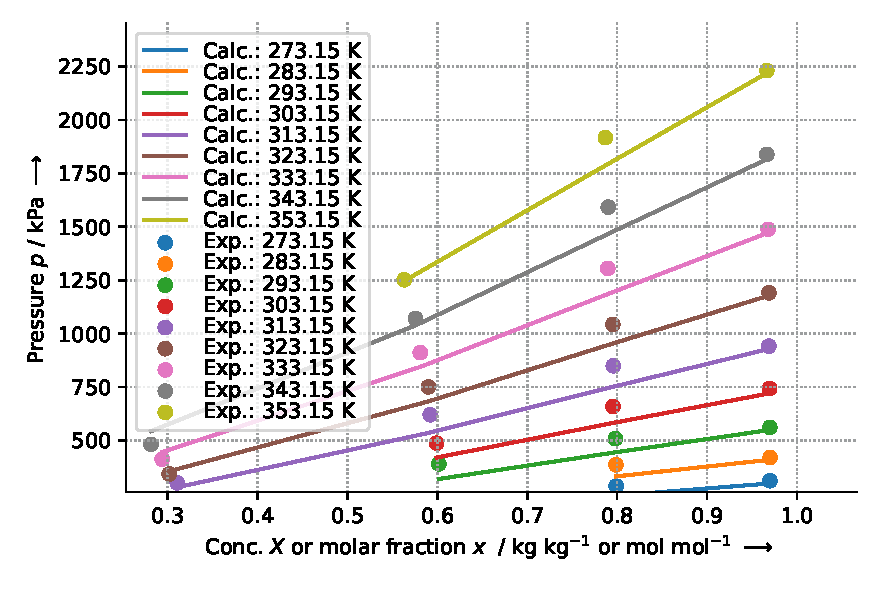
\includegraphics[height=10cm, keepaspectratio]{figs/abs/abs_R-12_paraffinic__NrtlFixedDg_1.pdf}}
\end{figure}
%

To generate the figure, the following refrigerant functions were selected:
\begin{itemize}
\item Vapor pressure: VaporPressure\_EoS1 - ID 1
\item Saturated liquid density: SaturatedLiquidDensity\_EoS1 - ID 1
\end{itemize}

The uncertainity of the experimental data is:
\begin{itemize}
\item Data source $\,\to\,$ Data was taken from figure
\item Pressure, absolute, in $\si{\pascal}$ $\,\to\,$ 3.45E+02
\item Temperature, absolute, in $\si{\kelvin}$ $\,\to\,$ 0.12
\end{itemize}

The mean absolute percentage error (MAPE) between the experimental and calculated data results in 7.29\%.
\FloatBarrier
\newpage
%%%%%%%%%%%%%%%%%%%%%%%%%%%%%%%%%%%%%%%%%%%%%%%%%%%%%%%%%%%%%%%%%%%%%%%%%%%%%%%
%%%%%%%%%%%%%%%%%%%%%%%%%%%%%%%%%%%%%%%%%%%%%%%%%%%%%%%%%%%%%%%%%%%%%%%%%%%%%%%
\subsubsection{TsubokaKatayama - ID 1}
%
\begin{tabular}[l]{|lp{11.5cm}|}
\hline
\addlinespace

\textbf{Sorbent:} & paraffinic \\
\textbf{Subtype:} &  \\
\textbf{Refrigerant:} & R-12 \\
\textbf{Equation:} & TsubokaKatayama \\
\textbf{ID:} & 1 \\
\textbf{Reference:} & Grebner, J. J. (1992): The Effects of Oil on the Thermodynamic Properties of Dichlorodifluoromethane (R-12) and Tetrafluoroethane (R-134a). Hg. v. Air Conditioning and Refrigeration Center. College of Engineering. University of Illinois at Urbana-Champaign. Air Conditioning and Refrigeration Center TR-13. Online verfügbar unter http://hdl.handle.net/2142/9702. \\
\textbf{Comment:} & See original literature: Use low-level interface to input molar volumes of both components, which are calculated by propper equations of state (i.e., v\_POE =  1/((55.37-0.020428*((T-273.15)*1.8+32))*16.0185)*0.5 in m3/mol), for calculations. \\

\addlinespace
\hline
\end{tabular}
\newline

\textbf{Equation and parameters:}
\newline
%
Pressure $p$ in $\si{\pascal}$ is calculated depending on molar fraction of refrigerant in the liquid phase $x_1$ in $\si{\mole\per\mole}$, temperature $T$ in $\si{\kelvin}$, molar volumes of both components ($v_1$ and $v_2$) in $\si{\cubic\meter\per\mole}$, and vapor pressure $p_\mathrm{sat,1}$ in $\si{\pascal}$. If molar volumes less than zero are used as function arguements, constant molar volumes given by parameter record are used. Equilibrium equation is given by:
%
\begin{equation*}
\begin{split}
p &=& \gamma_1 x_1 p_\mathrm{sat,1} & \quad\text{, and} \\
\gamma_1 &=& \exp \left( - \ln \left( x_1 + \Lambda_{21} x_2 \right) + x_2 \left( \frac{\Lambda_{21}}{x_1 + \Lambda_{21} x_2} - \frac{\Lambda_{12}}{x_1 \Lambda_{12} + x_2} \right) + \Phi \right) & \quad\text{, and} \\
\Phi &=& \ln \left( x_1 + x_2 \rho_{21} \right) - x_2 \left( \frac{\rho_{21}}{x_1 + x_2 \rho_{21}} - \frac{\rho_{12}}{x_1 \rho_{12} + x_2} \right) & \quad\text{, and} \\
\Lambda_{12} &=& \rho_{21} \exp \left( - \nicefrac{\Delta\lambda_{12}}{R T} \right) & \quad\text{, and} \\
\Lambda_{21} &=& \rho_{12} \exp \left( - \nicefrac{\Delta\lambda_{21}}{R T} \right) & \quad\text{, and} \\
\rho_{12} &=& \nicefrac{v_1}{v_2} & \quad\text{, and} \\
\rho_{21} &=& \nicefrac{v_2}{v_1} & \quad\text{, and} \\
x_2 &=& 1 - x_1  & \quad\text{.} \\
\end{split}
\end{equation*}
%
The parameters of the equation are:
%
\begin{longtable}[l]{lll|lll}
\toprule
\addlinespace
\textbf{Par.} & \textbf{Unit} & \textbf{Value} &	\textbf{Par.} & \textbf{Unit} & \textbf{Value} \\
\addlinespace
\midrule
\endhead

\bottomrule
\endfoot
\bottomrule
\endlastfoot
\addlinespace

$\Delta\lambda_{12}$ & $\si{\joule\per\mole}$ & 1.847000000e+03 & $\Delta\lambda_{21}$ & $\si{\joule\per\mole}$ & -4.437000000e+03 \\
$v_1$ & $\si{\cubic\meter\per\mole}$ & 1.000000000e+00 & $v_2$ & $\si{\cubic\meter\per\mole}$ & 1.000000000e+00 \\

\addlinespace\end{longtable}

\textbf{Validity:}
\newline
Equation is approximately valid for $255.15 \si{\kelvin} \leq T \leq 394.15 \si{\kelvin}$.
\newline

\textbf{Visualization:}
%
\begin{figure}[!htp]
{\noindent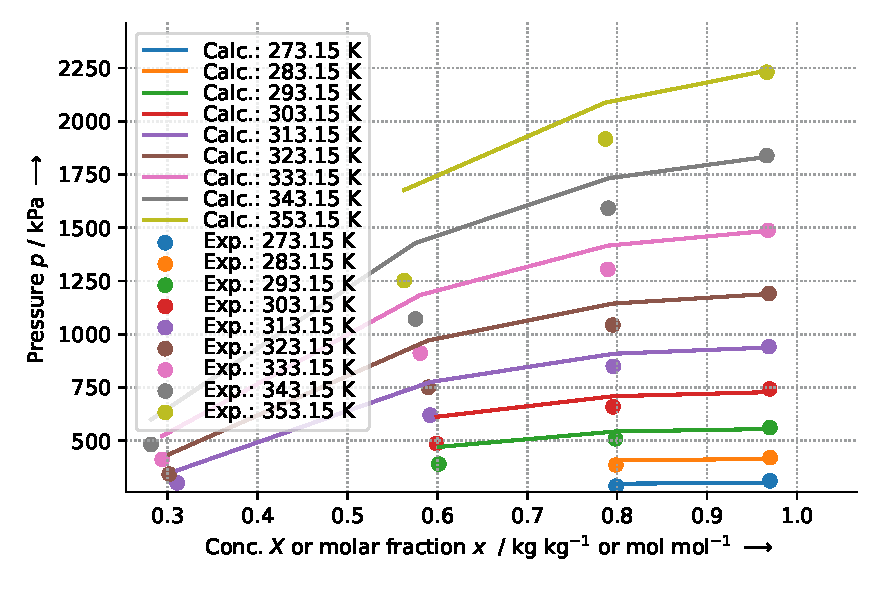
\includegraphics[height=10cm, keepaspectratio]{figs/abs/abs_R-12_paraffinic__TsubokaKatayama_1.pdf}}
\end{figure}
%

To generate the figure, the following refrigerant functions were selected:
\begin{itemize}
\item Vapor pressure: VaporPressure\_EoS1 - ID 1
\item Saturated liquid density: SaturatedLiquidDensity\_EoS1 - ID 1
\item Special refrigerant functions as described by comment and CoolProp
\end{itemize}

The uncertainity of the experimental data is:
\begin{itemize}
\item Data source $\,\to\,$ Data was taken from figure
\item Pressure, absolute, in $\si{\pascal}$ $\,\to\,$ 3.45E+02
\item Temperature, absolute, in $\si{\kelvin}$ $\,\to\,$ 0.12
\end{itemize}

The mean absolute percentage error (MAPE) between the experimental and calculated data results in 12.79\%.
\FloatBarrier
\newpage
%%%%%%%%%%%%%%%%%%%%%%%%%%%%%%%%%%%%%%%%%%%%%%%%%%%%%%%%%%%%%%%%%%%%%%%%%%%%%%%
%%%%%%%%%%%%%%%%%%%%%%%%%%%%%%%%%%%%%%%%%%%%%%%%%%%%%%%%%%%%%%%%%%%%%%%%%%%%%%%
\subsubsection{UniquacFixedDu - ID 1}
%
\begin{tabular}[l]{|lp{11.5cm}|}
\hline
\addlinespace

\textbf{Sorbent:} & paraffinic \\
\textbf{Subtype:} &  \\
\textbf{Refrigerant:} & R-12 \\
\textbf{Equation:} & UniquacFixedDu \\
\textbf{ID:} & 1 \\
\textbf{Reference:} & Grebner, J. J. (1992): The Effects of Oil on the Thermodynamic Properties of Dichlorodifluoromethane (R-12) and Tetrafluoroethane (R-134a). Hg. v. Air Conditioning and Refrigeration Center. College of Engineering. University of Illinois at Urbana-Champaign. Air Conditioning and Refrigeration Center TR-13. Online verfügbar unter http://hdl.handle.net/2142/9702. \\
\textbf{Comment:} & None \\

\addlinespace
\hline
\end{tabular}
\newline

\textbf{Equation and parameters:}
\newline
%
Pressure $p$ in $\si{\pascal}$ is calculated depending on molar fraction of refrigerant in the liquid phase $x_1$ in $\si{\mole\per\mole}$, temperature $T$ in $\si{\kelvin}$, and vapor pressure $p_\mathrm{sat,1}$ in $\si{\pascal}$ by:
%
\begin{equation*}
\begin{split}
p &=& \gamma_1 x_1 p_\mathrm{sat,1} & \quad\text{, and} \\
\gamma_1 &=& \exp \left( \ln \left( \nicefrac{\Phi_1}{x_1} \right) + q_1 \nicefrac{z}{2} \ln \left( \nicefrac{\Theta_1}{\Phi_1} \right) + l_1 - \nicefrac{\Phi_1}{x_2} \left( x_1 l_1 + x_2 l_2 \right) + \Gamma \right) & \quad\text{, and} \\
\Gamma &=& - q_1 \ln \left( \Theta_1 + \Theta_2 \tau_{21} \right) + q_1 - q_1 \left( \frac{\Theta_1}{\Theta_1 + \Theta_2 \tau_{21}} + \frac{\Theta_2 \tau_{12}}{\Theta_1 \tau_{12} + \Theta_2} \right) & \quad\text{, and} \\
\tau_{ij} &=& \exp \left( \nicefrac{\Delta u_{ij}}{R T} \right) & \quad\text{, and} \\
l_i &=& \nicefrac{z}{2} \left( r_i - q_i \right) \left(r_i - 1 \right) & \quad\text{, and} \\
\Theta_i &=& \frac{q_i x_i}{\sum_{j=1}^{2} q_j x_j} & \quad\text{, and} \\
\Phi_i &=& \frac{r_i x_i}{\sum_{j=1}^{2} r_j x_j} & \quad\text{, and} \\
x_2 &=& 1 - x_1  & \quad\text{.} \\
\end{split}
\end{equation*}
%
The parameters of the equation are:
%
\begin{longtable}[l]{lll|lll}
\toprule
\addlinespace
\textbf{Par.} & \textbf{Unit} & \textbf{Value} &	\textbf{Par.} & \textbf{Unit} & \textbf{Value} \\
\addlinespace
\midrule
\endhead

\bottomrule
\endfoot
\bottomrule
\endlastfoot
\addlinespace

$\Delta u_{12}$ & $\si{\joule\per\mole}$ & 5.897000000e+03 & $\Delta u_{21}$ & $\si{\joule\per\mole}$ & 2.770000000e+02 \\
$r_{1}$ & - & 2.624300000e+00 & $r_{2}$ & - & 2.450000000e+01 \\
$q_{1}$ & - & 2.376000000e+00 & $q_{2}$ & - & 2.028000000e+01 \\
$z$ & - & 1.000000000e+01 & & &  \\

\addlinespace\end{longtable}

\textbf{Validity:}
\newline
Equation is approximately valid for $255.15 \si{\kelvin} \leq T \leq 394.15 \si{\kelvin}$.
\newline

\textbf{Visualization:}
%
\begin{figure}[!htp]
{\noindent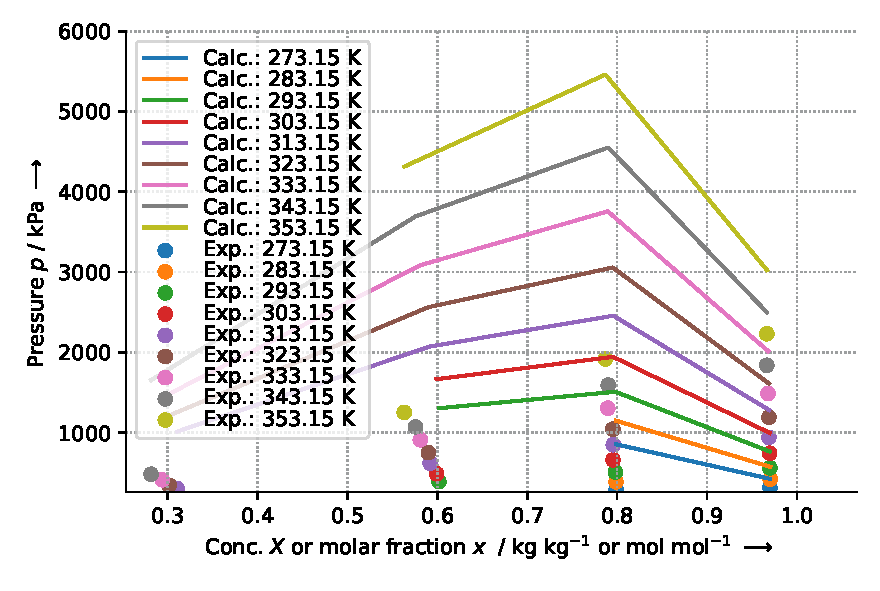
\includegraphics[height=10cm, keepaspectratio]{figs/abs/abs_R-12_paraffinic__UniquacFixedDu_1.pdf}}
\end{figure}
%

To generate the figure, the following refrigerant functions were selected:
\begin{itemize}
\item Vapor pressure: VaporPressure\_EoS1 - ID 1
\item Saturated liquid density: SaturatedLiquidDensity\_EoS1 - ID 1
\end{itemize}

The uncertainity of the experimental data is:
\begin{itemize}
\item Data source $\,\to\,$ Data was taken from figure
\item Pressure, absolute, in $\si{\pascal}$ $\,\to\,$ 3.45E+02
\item Temperature, absolute, in $\si{\kelvin}$ $\,\to\,$ 0.12
\end{itemize}

The mean absolute percentage error (MAPE) between the experimental and calculated data results in 162.47\%.
\FloatBarrier
\newpage
%%%%%%%%%%%%%%%%%%%%%%%%%%%%%%%%%%%%%%%%%%%%%%%%%%%%%%%%%%%%%%%%%%%%%%%%%%%%%%%
%%%%%%%%%%%%%%%%%%%%%%%%%%%%%%%%%%%%%%%%%%%%%%%%%%%%%%%%%%%%%%%%%%%%%%%%%%%%%%%
\subsubsection{WangChao - ID 1}
%
\begin{tabular}[l]{|lp{11.5cm}|}
\hline
\addlinespace

\textbf{Sorbent:} & paraffinic \\
\textbf{Subtype:} &  \\
\textbf{Refrigerant:} & R-12 \\
\textbf{Equation:} & WangChao \\
\textbf{ID:} & 1 \\
\textbf{Reference:} & Grebner, J. J. (1992): The Effects of Oil on the Thermodynamic Properties of Dichlorodifluoromethane (R-12) and Tetrafluoroethane (R-134a). Hg. v. Air Conditioning and Refrigeration Center. College of Engineering. University of Illinois at Urbana-Champaign. Air Conditioning and Refrigeration Center TR-13. Online verfügbar unter http://hdl.handle.net/2142/9702. \\
\textbf{Comment:} & See original literature: Use low-level interface to input molar volumes of both components, which are calculated by propper equations of state (i.e., v\_POE =  1/((55.37-0.020428*((T-273.15)*1.8+32))*16.0185)*0.5 in m3/mol), for calculations. \\

\addlinespace
\hline
\end{tabular}
\newline

\textbf{Equation and parameters:}
\newline
%
Pressure $p$ in $\si{\pascal}$ is calculated depending on molar fraction of refrigerant in the liquid phase $x_1$ in $\si{\mole\per\mole}$, temperature $T$ in $\si{\kelvin}$, molar volumes of both components ($v_1$ and $v_2$) in $\si{\cubic\meter\per\mole}$, and vapor pressure $p_\mathrm{sat,1}$ in $\si{\pascal}$. If molar volumes less than zero are used as function arguements, constant molar volumes given by parameter record are used. Equilibrium equation is given by:
%
\begin{equation*}
\begin{split}
p &=& \gamma_1 x_1 p_\mathrm{sat,1} & \quad\text{, and} \\
\gamma_1 &=& \exp \left( - \ln \left( x_1 + \Lambda_{21} x_2 \right) + x_2 \left( \frac{\Lambda_{21}}{x_1 + \Lambda_{21} x_2} - \frac{\Lambda_{12}}{x_1 \Lambda_{12} + x_2} \right) + \Phi \right) & \quad\text{, and} \\
\Phi &=& \frac{1}{R T} \frac{z}{2} \left( x_{21}^2 \Delta\lambda_{21} + x_2 x_{22} \frac{x_{12}}{x_1} \Delta\lambda_{12} \right) & \quad\text{, and} \\
x_{11} &=& \left( 1 + \nicefrac{x_2}{x_1} \exp \left( - \nicefrac{\Delta\lambda_{21}}{R T} \right) \right) ^ {-1} & \quad\text{, and} \\
x_{22} &=& \left( 1 + \nicefrac{x_1}{x_2} \exp \left( - \nicefrac{\Delta\lambda_{12}}{R T} \right) \right) ^ {-1} & \quad\text{, and} \\
\Lambda_{12} &=& \rho_{21} \exp \left( - \frac{\Delta\lambda_{12}}{R T} \right) & \quad\text{, and} \\
\Lambda_{21} &=& \rho_{12} \exp \left( - \frac{\Delta\lambda_{21}}{R T} \right) & \quad\text{, and} \\
\rho_{12} &=& \nicefrac{v_1}{v_2} & \quad\text{, and} \\
\rho_{21} &=& \nicefrac{v_2}{v_1} & \quad\text{, and} \\
x_{12} &=& 1 - x_{22} & \quad\text{, and} \\
x_{21} &=& 1 - x_{11} & \quad\text{, and} \\
x_2 &=& 1 - x_1  & \quad\text{.} \\
\end{split}
\end{equation*}
%
The parameters of the equation are:
%
\begin{longtable}[l]{lll|lll}
\toprule
\addlinespace
\textbf{Par.} & \textbf{Unit} & \textbf{Value} &	\textbf{Par.} & \textbf{Unit} & \textbf{Value} \\
\addlinespace
\midrule
\endhead

\bottomrule
\endfoot
\bottomrule
\endlastfoot
\addlinespace

$\Delta\lambda_{12}$ & $\si{\joule\per\mole}$ & -4.300000000e+01 & $\Delta\lambda_{21}$ & $\si{\joule\per\mole}$ & 4.115000000e+03 \\
$v_1$ & $\si{\cubic\meter\per\mole}$ & 1.000000000e+00 & $v_2$ & $\si{\cubic\meter\per\mole}$ & 1.000000000e+00 \\
$z$ & - & 6.000000000e+00 & & & \\

\addlinespace\end{longtable}

\textbf{Validity:}
\newline
Equation is approximately valid for $255.15 \si{\kelvin} \leq T \leq 394.15 \si{\kelvin}$.
\newline

\textbf{Visualization:}
%
\begin{figure}[!htp]
{\noindent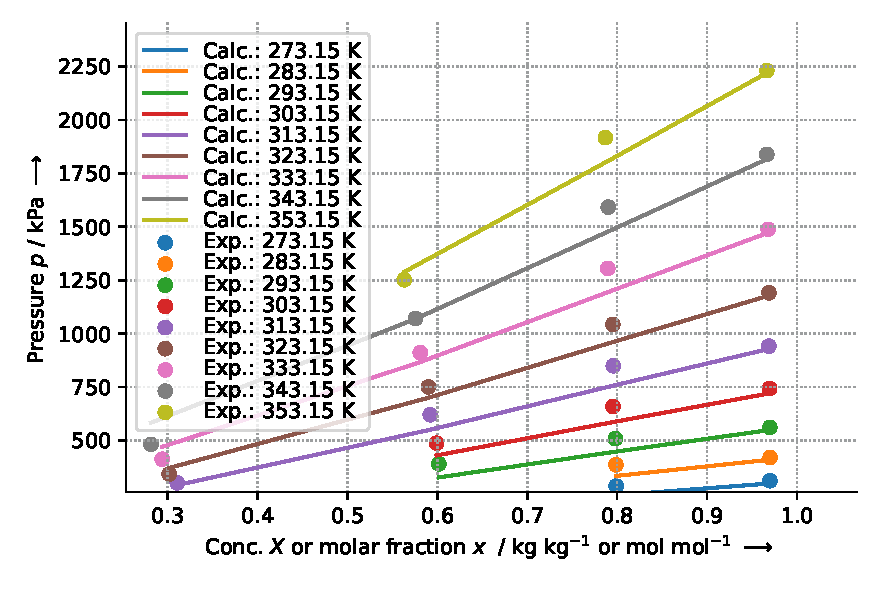
\includegraphics[height=10cm, keepaspectratio]{figs/abs/abs_R-12_paraffinic__WangChao_1.pdf}}
\end{figure}
%

To generate the figure, the following refrigerant functions were selected:
\begin{itemize}
\item Vapor pressure: VaporPressure\_EoS1 - ID 1
\item Saturated liquid density: SaturatedLiquidDensity\_EoS1 - ID 1
\item Special refrigerant functions as described by comment and CoolProp
\end{itemize}

The uncertainity of the experimental data is:
\begin{itemize}
\item Data source $\,\to\,$ Data was taken from figure
\item Pressure, absolute, in $\si{\pascal}$ $\,\to\,$ 3.45E+02
\item Temperature, absolute, in $\si{\kelvin}$ $\,\to\,$ 0.12
\end{itemize}

The mean absolute percentage error (MAPE) between the experimental and calculated data results in 7.23\%.
\FloatBarrier
\newpage
%%%%%%%%%%%%%%%%%%%%%%%%%%%%%%%%%%%%%%%%%%%%%%%%%%%%%%%%%%%%%%%%%%%%%%%%%%%%%%%
%%%%%%%%%%%%%%%%%%%%%%%%%%%%%%%%%%%%%%%%%%%%%%%%%%%%%%%%%%%%%%%%%%%%%%%%%%%%%%%
\subsubsection{WilsonFixedDl - ID 1}
%
\begin{tabular}[l]{|lp{11.5cm}|}
\hline
\addlinespace

\textbf{Sorbent:} & paraffinic \\
\textbf{Subtype:} &  \\
\textbf{Refrigerant:} & R-12 \\
\textbf{Equation:} & WilsonFixedDl \\
\textbf{ID:} & 1 \\
\textbf{Reference:} & Grebner, J. J. (1992): The Effects of Oil on the Thermodynamic Properties of Dichlorodifluoromethane (R-12) and Tetrafluoroethane (R-134a). Hg. v. Air Conditioning and Refrigeration Center. College of Engineering. University of Illinois at Urbana-Champaign. Air Conditioning and Refrigeration Center TR-13. Online verfügbar unter http://hdl.handle.net/2142/9702. \\
\textbf{Comment:} & See original literature: Use low-level interface to input molar volumes of both components, which are calculated by propper equations of state (i.e., v\_POE =  1/((55.37-0.020428*((T-273.15)*1.8+32))*16.0185)*0.5 in m3/mol), for calculations. \\

\addlinespace
\hline
\end{tabular}
\newline

\textbf{Equation and parameters:}
\newline
%
Pressure $p$ in $\si{\pascal}$ is calculated depending on molar fraction of refrigerant in the liquid phase $x_1$ in $\si{\mole\per\mole}$, temperature $T$ in $\si{\kelvin}$, molar volumes of both components ($v_1$ and $v_2$) in $\si{\cubic\meter\per\mole}$, and vapor pressure $p_\mathrm{sat,1}$ in $\si{\pascal}$. If molar volumes less than zero are used as function arguements, constant molar volumes given by parameter record are used. Equilibrium equation is given by:
%
\begin{equation*}
\begin{split}
p &=& \gamma_1 x_1 p_\mathrm{sat,1} & \quad\text{, and} \\
\gamma_1 &=& \exp \left( - \ln \left( x_1 + \Lambda_{12} x_2 \right) + x_2 \left( \frac{\Lambda_{12}}{x_1 + \Lambda_{12} x_2} - \frac{\Lambda_{21}}{x_2 + \Lambda_{21} x_1} \right) \right) & \quad\text{, and} \\
\Lambda_{12} &=& \begin{cases} \nicefrac{v_2}{v_1} \exp \left( - \nicefrac{\Delta\lambda_{12}}{R T} \right) & \quad \text{if } \Lambda_{12}^{*} = 0 \\ \Lambda_{12}^{*}  & \quad \text{else} \end{cases}  & \quad\text{, and} \\
\Lambda_{21} &=& \begin{cases} \nicefrac{v_1}{v_2} \exp \left( - \nicefrac{\Delta\lambda_{21}}{R T} \right) & \quad \text{if } \Lambda_{21}^{*} = 0 \\ \Lambda_{21}^{*}  & \quad \text{else} \end{cases}  & \quad\text{, and} \\
x_2 &=& 1 - x_1  & \quad\text{.} \\
\end{split}
\end{equation*}
%
The parameters of the equation are:
%
\begin{longtable}[l]{lll|lll}
\toprule
\addlinespace
\textbf{Par.} & \textbf{Unit} & \textbf{Value} &	\textbf{Par.} & \textbf{Unit} & \textbf{Value} \\
\addlinespace
\midrule
\endhead

\bottomrule
\endfoot
\bottomrule
\endlastfoot
\addlinespace

$\Lambda_{12}^{*}$ & - & 0.000000000e+00 & $\Lambda_{21}^{*}$ & - & 0.000000000e+00 \\
$\Delta\lambda_{12}$ & $\si{\joule\per\mole}$ & 2.634000000e+03 & $\Delta\lambda_{21}$ & $\si{\joule\per\mole}$ & 7.415000000e+03 \\
$v_1$ & $\si{\cubic\meter\per\mole}$ & 1.000000000e+00 & $v_2$ & $\si{\cubic\meter\per\mole}$ & 1.000000000e+00 \\

\addlinespace\end{longtable}

\textbf{Validity:}
\newline
Equation is approximately valid for $255.15 \si{\kelvin} \leq T \leq 394.15 \si{\kelvin}$.
\newline

\textbf{Visualization:}
%
\begin{figure}[!htp]
{\noindent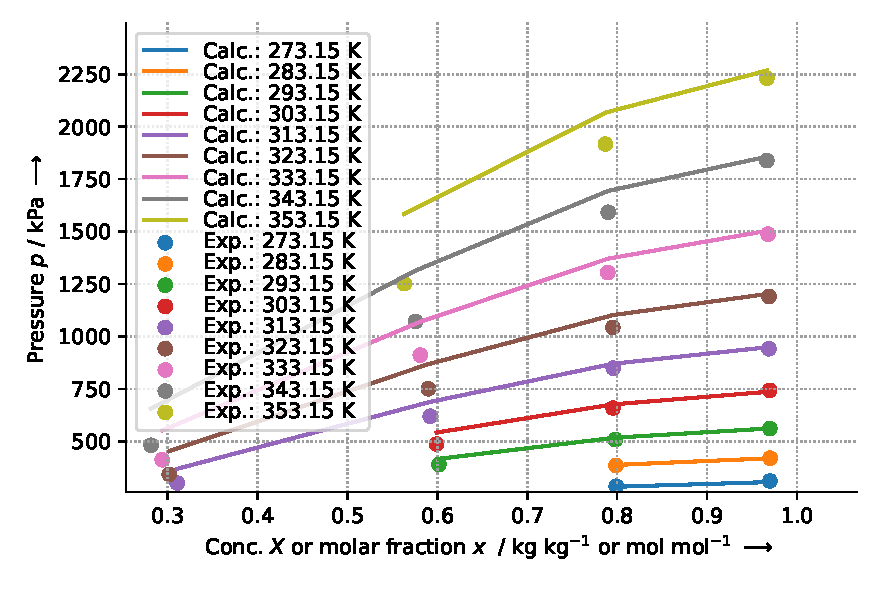
\includegraphics[height=10cm, keepaspectratio]{figs/abs/abs_R-12_paraffinic__WilsonFixedDl_1.pdf}}
\end{figure}
%

To generate the figure, the following refrigerant functions were selected:
\begin{itemize}
\item Vapor pressure: VaporPressure\_EoS1 - ID 1
\item Saturated liquid density: SaturatedLiquidDensity\_EoS1 - ID 1
\item Special refrigerant functions as described by comment and CoolProp
\end{itemize}

The uncertainity of the experimental data is:
\begin{itemize}
\item Data source $\,\to\,$ Data was taken from figure
\item Pressure, absolute, in $\si{\pascal}$ $\,\to\,$ 3.45E+02
\item Temperature, absolute, in $\si{\kelvin}$ $\,\to\,$ 0.12
\end{itemize}

The mean absolute percentage error (MAPE) between the experimental and calculated data results in 9.58\%.
\FloatBarrier
\newpage
%%%%%%%%%%%%%%%%%%%%%%%%%%%%%%%%%%%%%%%%%%%%%%%%%%%%%%%%%%%%%%%%%%%%%%%%%%%%%%%
